\chapter{Introducci�n}
\label{chapter:introduccion}


%%% SECTION
\section{Descripci�n general del problema}

En la actualidad, los procesos de miner�a de datos requieren grandes cantidades de datos, que en muchas ocasiones contienen informaci�n personal y privada de usuarios o personas. Aunque se realicen procesos b�sicos de anonimizaci�n sobre los datos, es decir, eliminaci�n de los nombres u otros identificadores clave, existen multitud de t�cnicas de re-identificaci�n que permiten volver a identificar a un usuario dentro de este conjunto de datos. En la Figura \ref{fig:context-anoni1} se presenta un mapa donde es posible contextualizar los procesos de anonimizaci�n y re-identificaci�n dentro de un proceso de miner�a de datos.

\begin{figure}
	\centering
	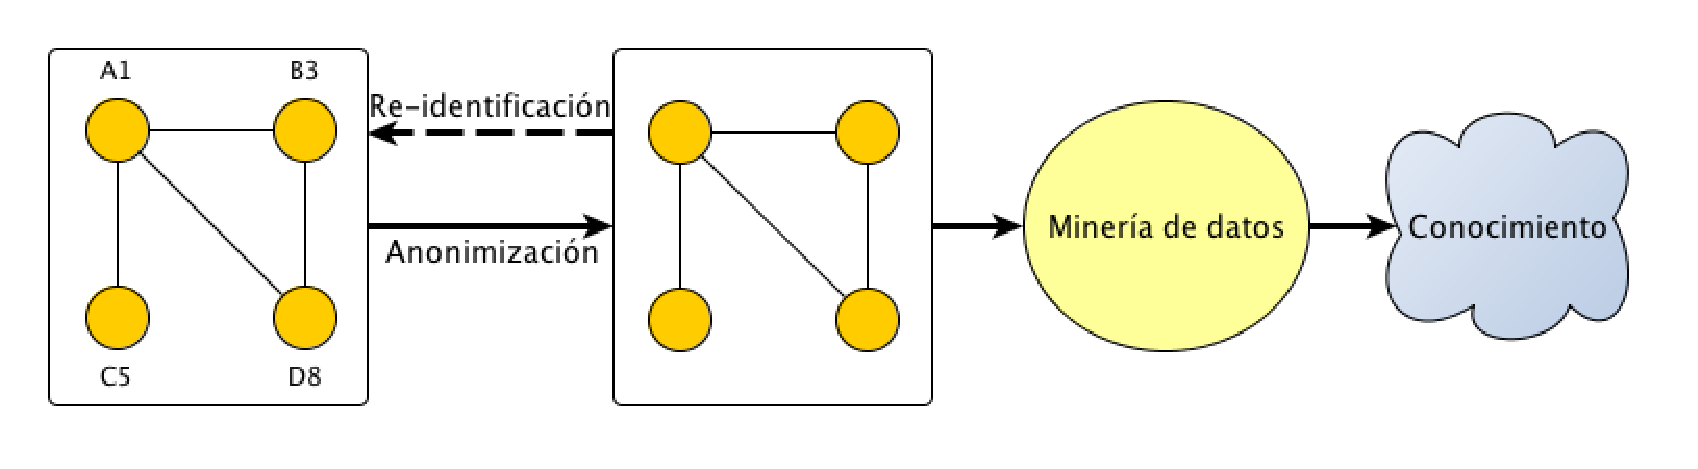
\includegraphics[width=0.8\textwidth]{figs/intro-1}
	\caption{Pie de la imagen.}
	\label{fig:context-anoni1}
\end{figure}

\subsection{Ejemplo de subsection}

Aunque se han realizado importantes avances en preservaci�n de la privacidad en publicaci�n de datos, tales como el modelo \textit{k}-anonymity \cite{Sweeney:2002}.

Un ejemplo de pseudo-c�digo se puede encontrar en el C�digo \ref{code:RandomSwitch-1}

\begin{algorithm}
	\caption{Pseudoc�digo del algoritmo \textit{Random Switch}}
	\label{code:RandomSwitch-1}
	\begin{algorithmic}
		\REQUIRE{El grafo original $G$ y el porcentaje de anonimizaci�n $p$ que se desea aplicar.}
		\ENSURE{El grafo $G$ anonimizado.}
		\STATE $num = round(G.num\_edges() * p)$
		\STATE $i = 0$
		\WHILE {$i < num$}
		\STATE {$e_{1} = G.random\_edge()$}
		\STATE $e_{2} = G.random\_edge()$
		\STATE $new\_e_{1} = (e_{1}.origen, e_{2}.origen)$
		\STATE $new\_e_{2} = (e_{1}.destino, e_{2}.destino)$
		\IF {$!G.exist(new\_e_{1})$ \AND $!G.exist(new\_e_{2})$}
		\STATE $G.add\_edge(new\_e_{1})$
		\STATE $G.add\_edge(new\_e_{2})$
		\STATE $G.delete\_edge(e_{1})$
		\STATE $G.delete\_edge(e_{2})$
		\STATE $i=i+1$
		\ENDIF
		\ENDWHILE
		\RETURN $G$
	\end{algorithmic}
\end{algorithm}

Un ejemplo de tabla se puede ver en la Tabla \ref{table:ejemplo_vertex_refi_query}

\begin{table}
	\centering{}
	\begin{tabular}{ l || c | c | l }
		\hline
		Node ID & $\mathcal{H}_{0}$ & $\mathcal{H}_{1}$ & $\mathcal{H}_{2}$ \\
		\hline
		\hline
		Alice & $\epsilon$ & 1 & \{4\}  \\
		\hline
		Bob & $\epsilon$ & 4 & \{1, 1, 4, 4\}  \\
		\hline
		Carol & $\epsilon$ & 1 & \{4\}  \\
		\hline
		Dave & $\epsilon$ & 4 & \{2, 4, 4, 4\}  \\
		\hline
		Ed & $\epsilon$ & 4 & \{2, 4, 4, 4\}  \\
		\hline
		Fred & $\epsilon$ & 2 & \{4, 4\}  \\
		\hline
		Greg & $\epsilon$ & 4 & \{2, 2, 4, 4\}  \\
		\hline
		Harry & $\epsilon$ & 2 & \{4, 4\}  \\
		\hline
	\end{tabular}
	\caption{\textit{Vertex refinement queries}.}
	\label{table:ejemplo_vertex_refi_query}
\end{table}